\documentclass[a4paper, 12pt, addpoints]{exam}
\usepackage{IfbaListas}
\usepackage{pgfplots}
\pgfplotsset{compat=1.16}

\tikzset{
    cross/.pic = {
        \draw[ultra thick, rotate = 45] (-#1,0) -- (#1,0);
        \draw[ultra thick, rotate = 45] (0,-#1) -- (0, #1);
    }
}


\begin{document}

    \pagestyle{fancy}
    \fancyhead[RO]{Fundamentos de Física II, 2024}
    \fancyhead[L]{Alberto Aurensanz Clemente}


    \begin{center}
    \setlength\fboxsep{15px}
    \shadowbox{\parbox{0.52\textwidth}{
        \textbf{Declaración de Autoría}
        \\[15px]
        El alumno ALBERTO AURENSANZ CLEMENTE \href{mailto:aaurensan3@alumno.uned.es}{aaurensan3@alumno.uned.es},
        con DNI número 73090547C, declara que es el autor
        único e individual de este trabajo.

        \vspace{10px}
        Fdo:
        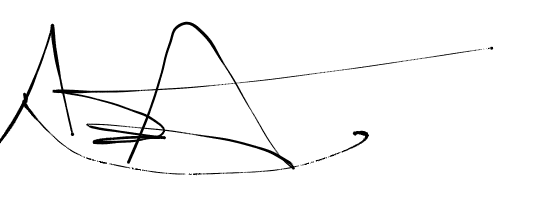
\includegraphics[scale=0.45]{files/signature}

    }}
\end{center}

    \vspace{20px}
    \textbf{CUESTIÓN}
\vspace{20px}

El campo eléctrico dentro de un conductor,

\begin{enumerate}[label=\alph*.]
    \item Es siempre cero.
    \item Es cero, excepto en el caso de que haya cargas fijas en algún punto del interior del conductor en cuyo caso
    no es cero.
    \item Es constante, pero no cero.
    \item Es cero, incluso en el caso de que haya cargas fijas en algún punto del interior del conductor.
\end{enumerate}

\vspace{20px}
\textit{Solución:}
\\

Empezamos considerando la situación de un conductor en equilibro electrostático sin cargas fijas en su interior. En ese caso,
el campo eléctrico dentro del conductor debe ser cero. Descartamos por tanto la opción $c$ como respuesta.\\

Consideramos ahora la situación en la que existen cargas fijas en algún punto del interior del conductor. Si aplicamos la ley de Gauss a una superficie
que contenga las cargas fijas y que esté contenida en su totalidad en el interior del conductor,  llegamos a la conclusión de
que el campo eléctrico en esa región no es cero, independientemente de la forma
que tenga esta superficie. Así, podemos descartar las respuestas $a$ y $d$.\\

Las cargas fijas en el interior del conductor inducen una carga de signo opuesto en la superficie interior del conductor.
Las cargas fijas y las inducidas dan como resultado un campo eléctrico nulo fuera de la superficie interior del conductor, pero
no así en la región interior. Por tanto, la respuesta correcta es la $b$.







    \newpage

    \textbf{1. Elaboración de tabla con todos los datos}

\vspace{20px}

Como punto de partida, se recogen los datos de desplazamiento espectral $z$, distancia $r$ (Mpc) y Magnitud aparente visual $m_v$ del software
Stellarium.

La Magnitud absoluta visual $M_v$ se calcula a partir de la Magnitud aparente visual gracias a la relación:

\begin{equation*}
    m - M = 5 \log\frac{r[\text{pc}]}{10} = 5 \log r[\text{pc}] - 5,
\end{equation*}

que equivale a desplazar la galaxia a una distancia estándar de $r$ = 10 pc y medir allí su brillo.

La velocidad de recesión $v$ y la constante de Hubble $H_0$ se obtienen de la relación:

\begin{equation*}
    v = c\,z = H_0\,r,
    \end{equation*}

que nos indica que el desplazamiento espectral $z$ se incrementa con la distancia $r$ de la galaxia, y que existe una relación lineal entre su
distancia y velocidad de recesión.\\

Para hacer los cálculos de las magnitudes mencionadas, se obvian los márgenes de error que nos proporciona Stellarium, aunque sí que se que han
recogido en la tabla pedida.

Los valores numéricos se muestran con delimitadores en notación inglesa.

\begin{table}[H]
    \scriptsize
    \begin{tabular}{|p{64px}|p{80px}|p{57px}|p{54px}|p{54px}|p{54px}|p{60px}|}
        \hline
        \textbf{Identificador de la galaxia} & \textbf{Desplazamiento espectral $z$} & \textbf{Distancia $r$ (Mpc)} & \textbf{Velocidad de recesión $v$ (km/s)}
        & \textbf{Magnitud aparente visual $m_v$} & \textbf{Magnitud absoluta visual $M_v$} & \textbf{Constante de Hubble $H_0$ (km/s Mpc)} \\
        \hline
        \csvreader[late after line=\\]{files/data.csv}{}% use head of csv as column names
        {\csvcoli&\csvcolii&\csvcoliii&\csvcoliv&\csvcolv&\csvcolvi&\csvcolvii}% specify your columns here
        \hline
    \end{tabular}
\end{table}




    \newpage
    \textbf{PROBLEMA 2}
\vspace{20px}

\newcommand{\ivec}{\boldsymbol{\hat{\imath}}}
\newcommand{\jvec}{\boldsymbol{\hat{\jmath}}}
\newcommand{\kvec}{\boldsymbol{\hat{k}}}

Tres alambres infinitos paralelos entre sı́ y perpendiculares al plano de la hoja se ubican en los vértices de
un cuadrado de lado $d$. Uno de ellos lleva corriente $2I$ que entra al plano, mientras que los otros llevan corriente
$I$ que emerge del plano de la hoja.\\

\begin{enumerate}[label=\alph*.]
    \item Calcule el vector campo magnético en el punto $P_1$.
    \item Calcule la fuerza que actúa sobre una carga $q$ con velocidad $\mathbf{v} = 3 \ivec
    + 2 \jvec  + \kvec$̃ situada en $P_1$.
    \item Supongamos que se traslada una carga desde el punto $P_1$ al punto $P_2$ a lo largo de la lı́nea recta que une
    esos dos puntos, ¿cuál es el trabajo que cuesta dicho traslado?
\end{enumerate}

\begin{center}
    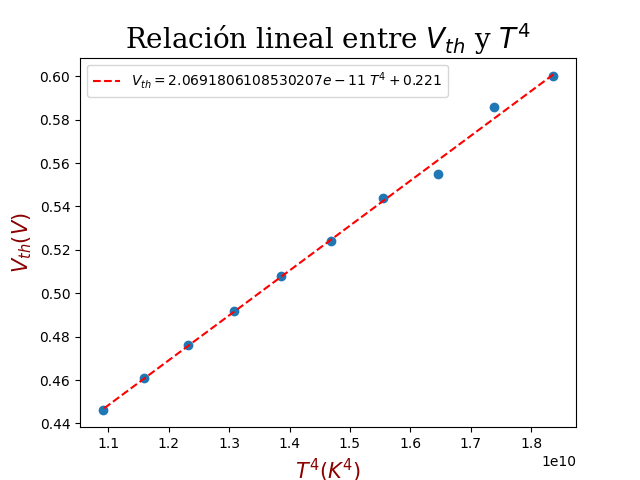
\includegraphics[width=10cm]{files/img2}
\end{center}

\vspace{20px}
\textit{Solución:}
\\

\textbf{a}. De acuerdo al principio de superposición, el campo magnético en el punto $P_1$ será la suma del campo magnético generado
por cada uno de los alambres. Podríamos calcular la contribución de cada alambre mediante la ley de Biot y Savart,
pero considerando la simetría del problema, y que los alambres son infinitos, es más fácil obtener la solución a partir de la ley
de Ampère.\\

\begin{equation*}
    \[ \oint_C \vec{B} \cdot d\vec{\ell} = \mu_{0}I_C \]
\end{equation*}


El campo magnético es constante a la largo de una curva circular por cuyo centro pasa el alambre, y su dirección es tangente a esta
circunferencia. Su módulo es $B = \frac{\mu_{0}I_C }{2\pi R}$. En la siguiente figura se representan los 3 campos magnéticos con sus
direcciones respectivas.


\begin{center}
    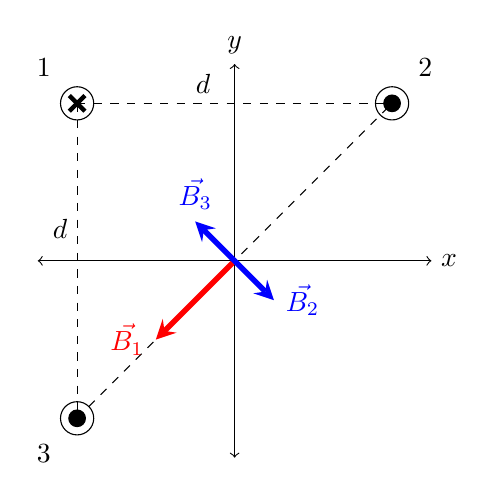
\begin{tikzpicture}
%    \draw[thin,gray!40] (-2,-2) grid (2,2);
        \draw[<->] (-2.5,0)--(2.5,0) node[right]{$x$};
        \draw[<->] (0,-2.5)--(0,2.5) node[above]{$y$};

        \draw[dashed] (-2,2)--(2,2) node[above,xshift=-2.4cm] {$d$};
        \draw[dashed] (-2,2)--(-2,-2) node[left,yshift=2.4cm] {$d$};;
        \draw[dashed] (-2,-2)--(2,2);



        \draw (-2,2) circle (6pt) node[above left=6pt]{$\boldsymbol{1}$};
        \draw (-2,2) pic[rotate = 0] {cross=4pt};

        \draw (2,2) circle (6pt) node[above right=6pt]{$\boldsymbol{2}$};
        \filldraw (2,2) circle (3pt);

        \draw (-2,-2) circle (6pt) node[below left=6pt]{$\boldsymbol{3}$};
        \filldraw (-2,-2) circle (3pt);


        \draw[line width=2pt,red,-stealth](0,0)--(-1,-1) node[anchor=east]{$\boldsymbol{\vec{B_1}}$};
        \draw[line width=2pt,blue,-stealth](0,0)--(0.5,-0.5) node[anchor=west]{$\boldsymbol{\vec{B_2}}$};
        \draw[line width=2pt,blue,-stealth](0,0)--(-0.5,0.5) node[anchor=south]{$\boldsymbol{\vec{B_3}}$};
    \end{tikzpicture}
\end{center}

La distancia de cada alambre al punto $P_1$ es $d / \sqrt{2}$. Observamos que los campos $\boldsymbol{\vec{B_}}_2$ y $\boldsymbol{\vec{B}}_3$ se cancelan por tener direcciones opuestas
y mismo módulo, por lo que el campo en el punto $P_1$ es $\boldsymbol{\vec{B}}_1$ .


\begin{equation*}
    \boldsymbol{\vec{B}}_{P1} = \boldsymbol{\vec{B}}_1 = \frac{\mu_{0} 2 I \sqrt{2} }{2 \pi d} \left( -\cos(45\degree )\ivec -\sen(45\degree)\jvec \right)
    = \frac{\mu_{0} I}{\pi d} \left( -\ivec -\jvec \right)
\end{equation*}


\textbf{b}. La fuerza de Lorentz describe la fuerza que actúa sobre una carga puntual en movimiento en presencia de un campo magnético.

\begin{equation*}
    \boldsymbol{\vec{F}} = q \boldsymbol{\vec{v}} \times \boldsymbol{\vec{B}}
\end{equation*}

Conocemos tanto $\boldsymbol{\vec{v}}$ como $\boldsymbol{\vec{B}}$, por lo que podemos realizar el producto vectorial para calcular la fuerza
que actúa sobre la carga $q$.

\begin{equation*}
    \boldsymbol{\vec{F}} = q \; \frac{\mu_{0} I}{\pi d} \left[(3 \ivec
    + 2 \jvec  + \kvec)  \times \left( -\ivec -\jvec \right)  \right] =
    \frac{\mu_{0} q I}{\pi d} (\ivec - \jvec - \kvec )
\end{equation*}

\textbf{c}. La fuerza magnética que actúa sobre una partícula cargada que se mueve a través de un campo magnético es siempre perpendicular a la
velocidad de la partícula. La fuerza magnética modifica la dirección de la velocidad, pero no su módulo. Por lo tanto,
los campos magnéticos no realizan trabajo sobre las partículas y no modifican su energía cinética. El trabajo que cuesta el traslado
de una carga desde el punto $P_1$ al punto $P_2$ es nulo.
    \newpage
    \textbf{PROBLEMA 3}
\vspace{20px}

En el circuito de la figura, los valores de las resistencias son $R_1 = 1\,\Omega$ y $R_2 = 100\,\Omega$. Sin embargo,
desconocemos la fuerza electromotriz de la fuente de tensión y la capacidad del condensador. Suponga en todo
momento que la fuente de tensión es ideal (su resistencia interna es despreciable).

\begin{enumerate}[label=\alph*.]
    \item Suponga que, inicialmente, el condensador está completamente descargado. En un momento determinado,
    situamos el interruptor en la posición $A$, conectando la fuente $\mathcal{E}$ y formando un circuito $RC$ con la
    resistencia $R_1$ y el condensador. Con un osciloscopio, medimos el voltaje entre las placas del condensador
    en función del tiempo, $v_C (t)$ y obtenemos, para los instantes previos y posteriores a la conexión de la
    fuente, la curva de la figura. Sabiendo que cada división del eje vertical representa 5\,V, deduzca la fuerza
    electromotriz de la fuente explicando brevemente su razonamiento.
    \item Desconocemos la capacidad del condensador, pero en el laboratorio solo tenemos condensadores de tres
    capacidades, 5\,$\mu$F, 5\,mF y 5\,F, por lo que el condensador del circuito debe ser alguno de estos tres. Sabiendo
    que cada división del eje horizontal de la gráfica representa 5\,s, deduzca la capacidad del condensador
    empleado en el circuito, explicando brevemente su razonamiento.
    \item Suponga que mantenemos el interruptor en la posición $A$ durante un tiempo muy largo, de modo que
    el condensador se carga por completo. En un instante posterior, al que nos referiremos como $t = 0$,
    cambiamos el interruptor a la posición $B$, desconectando la fuente de tensión y conectando el condensador
    a la resistencia $R_2$. Encuentre la expresión para la corriente que circula por la resistencia $R_2$ en función
    del tiempo para $t > 0$.
    \item Si mantenemos el interruptor en la posición $B$ durante un tiempo indefinido, calcule, por el procedimiento
    que considere más adecuado, la energı́a total que disipa la resistencia $R_2$ entre $t = 0$ y $t\;$\rightarrow$ \infty$.
\end{enumerate}

\begin{center}
    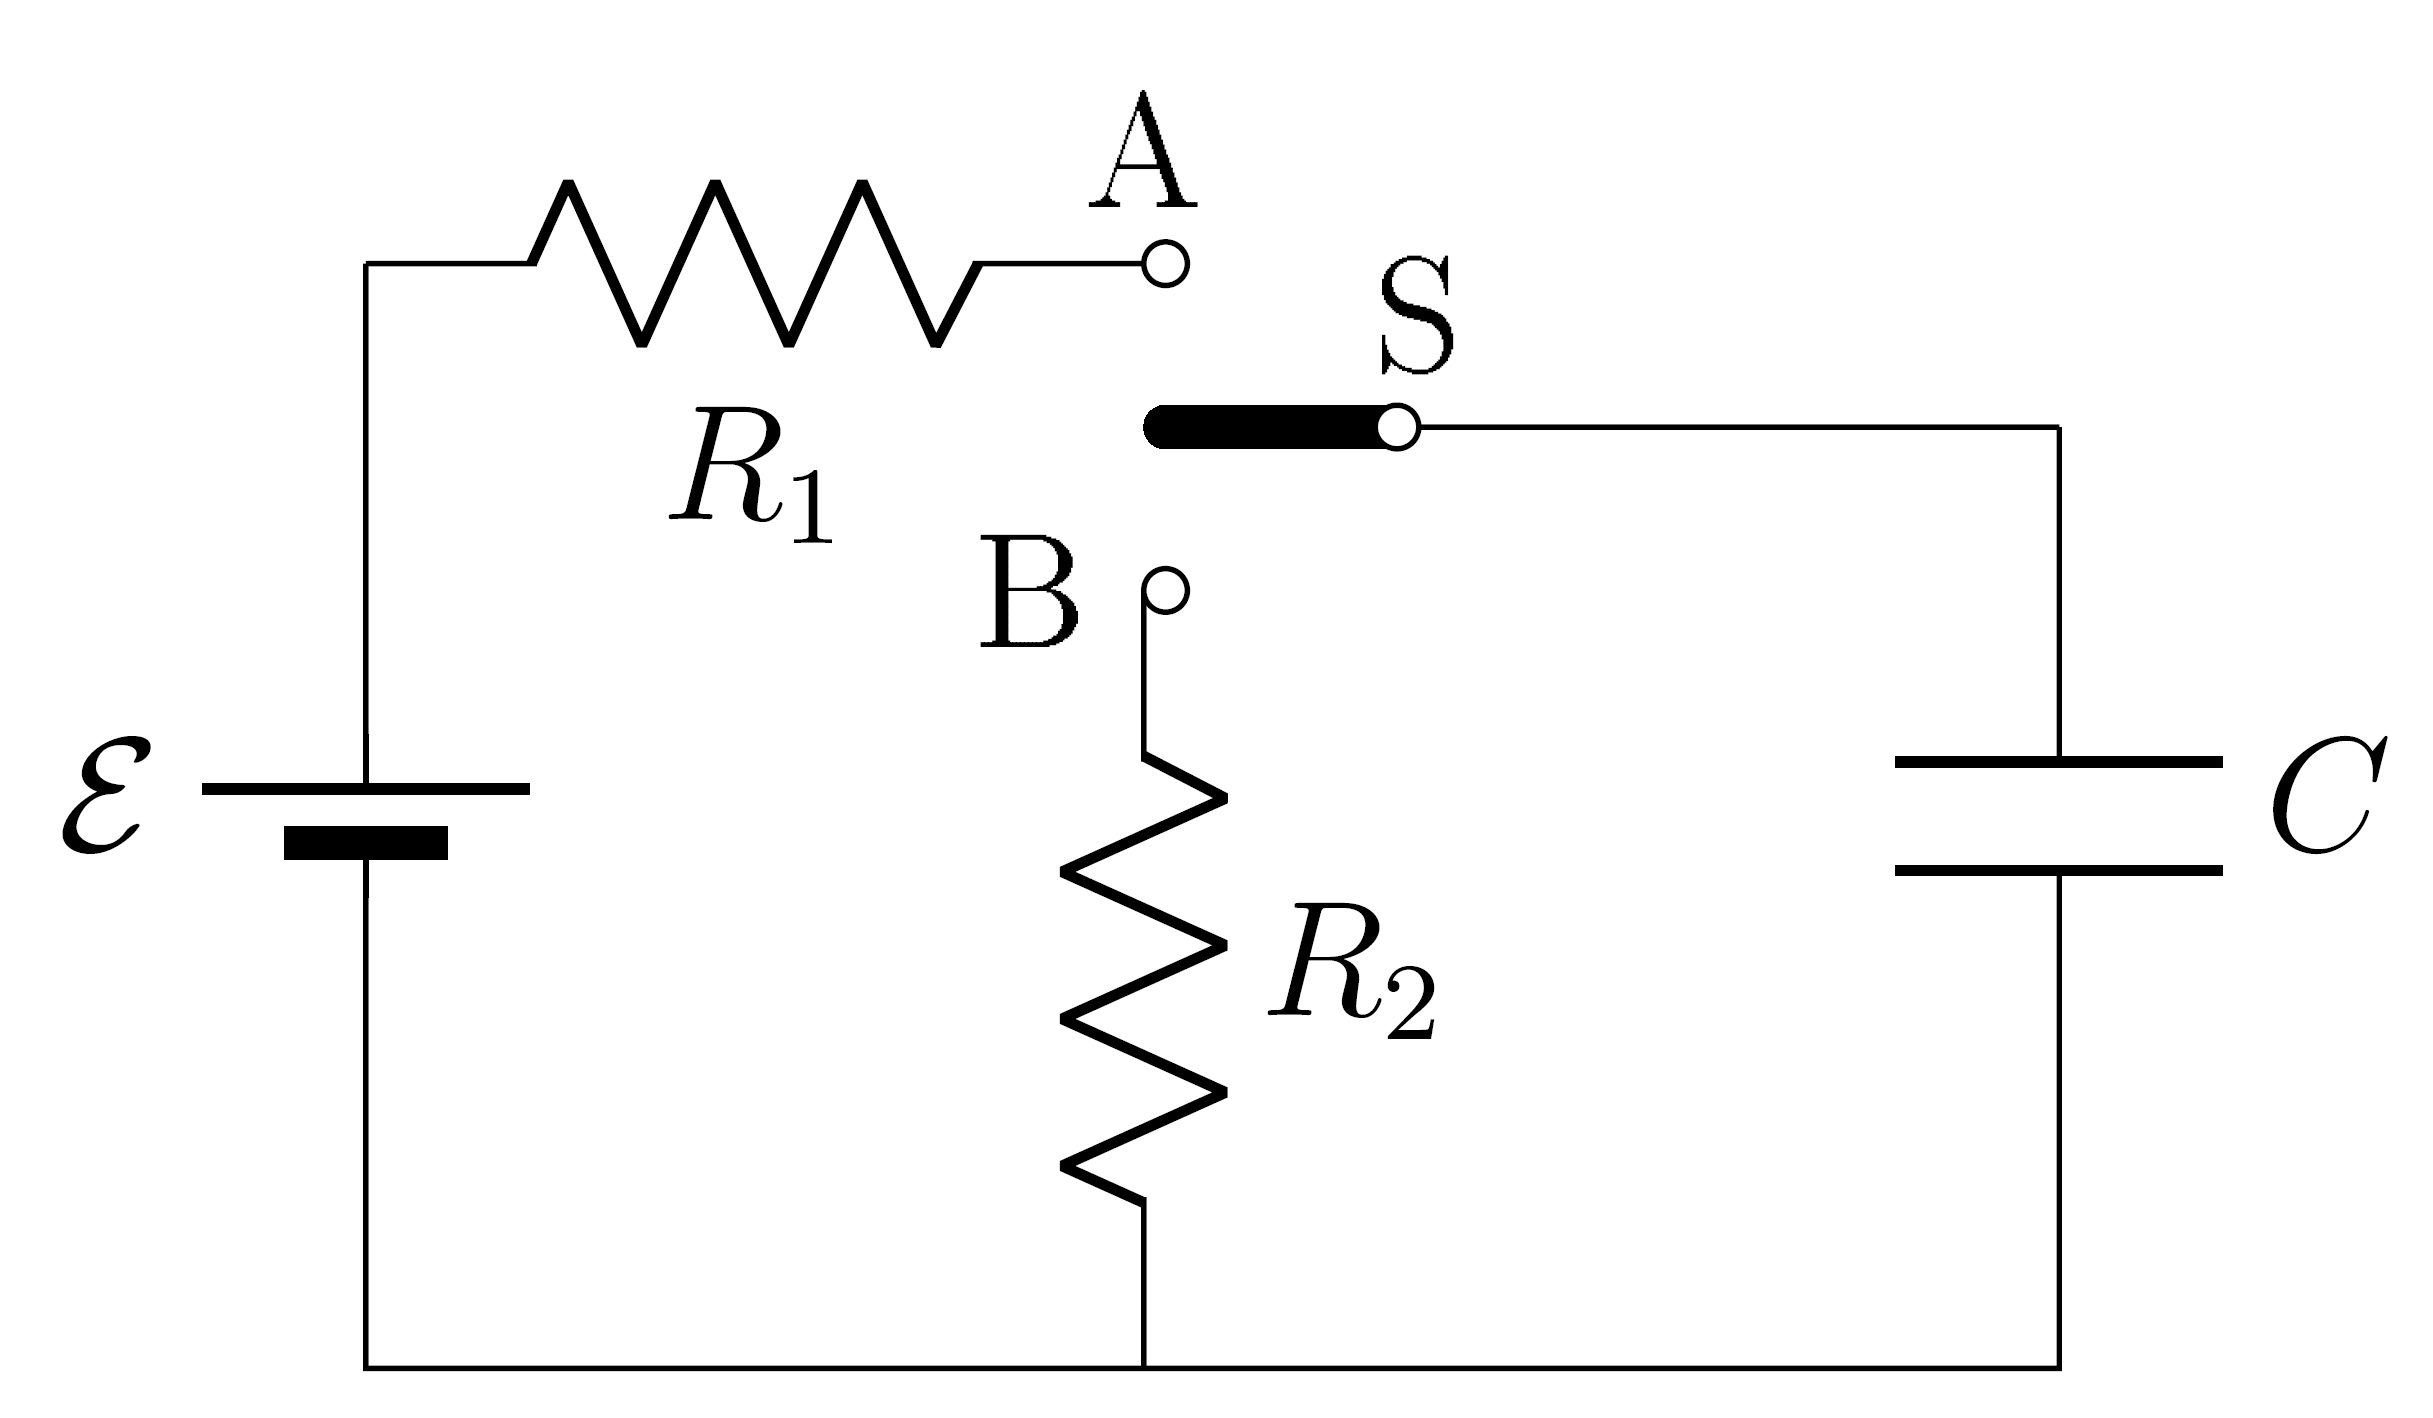
\includegraphics[width=12cm]{files/img3}
\end{center}
\begin{center}
    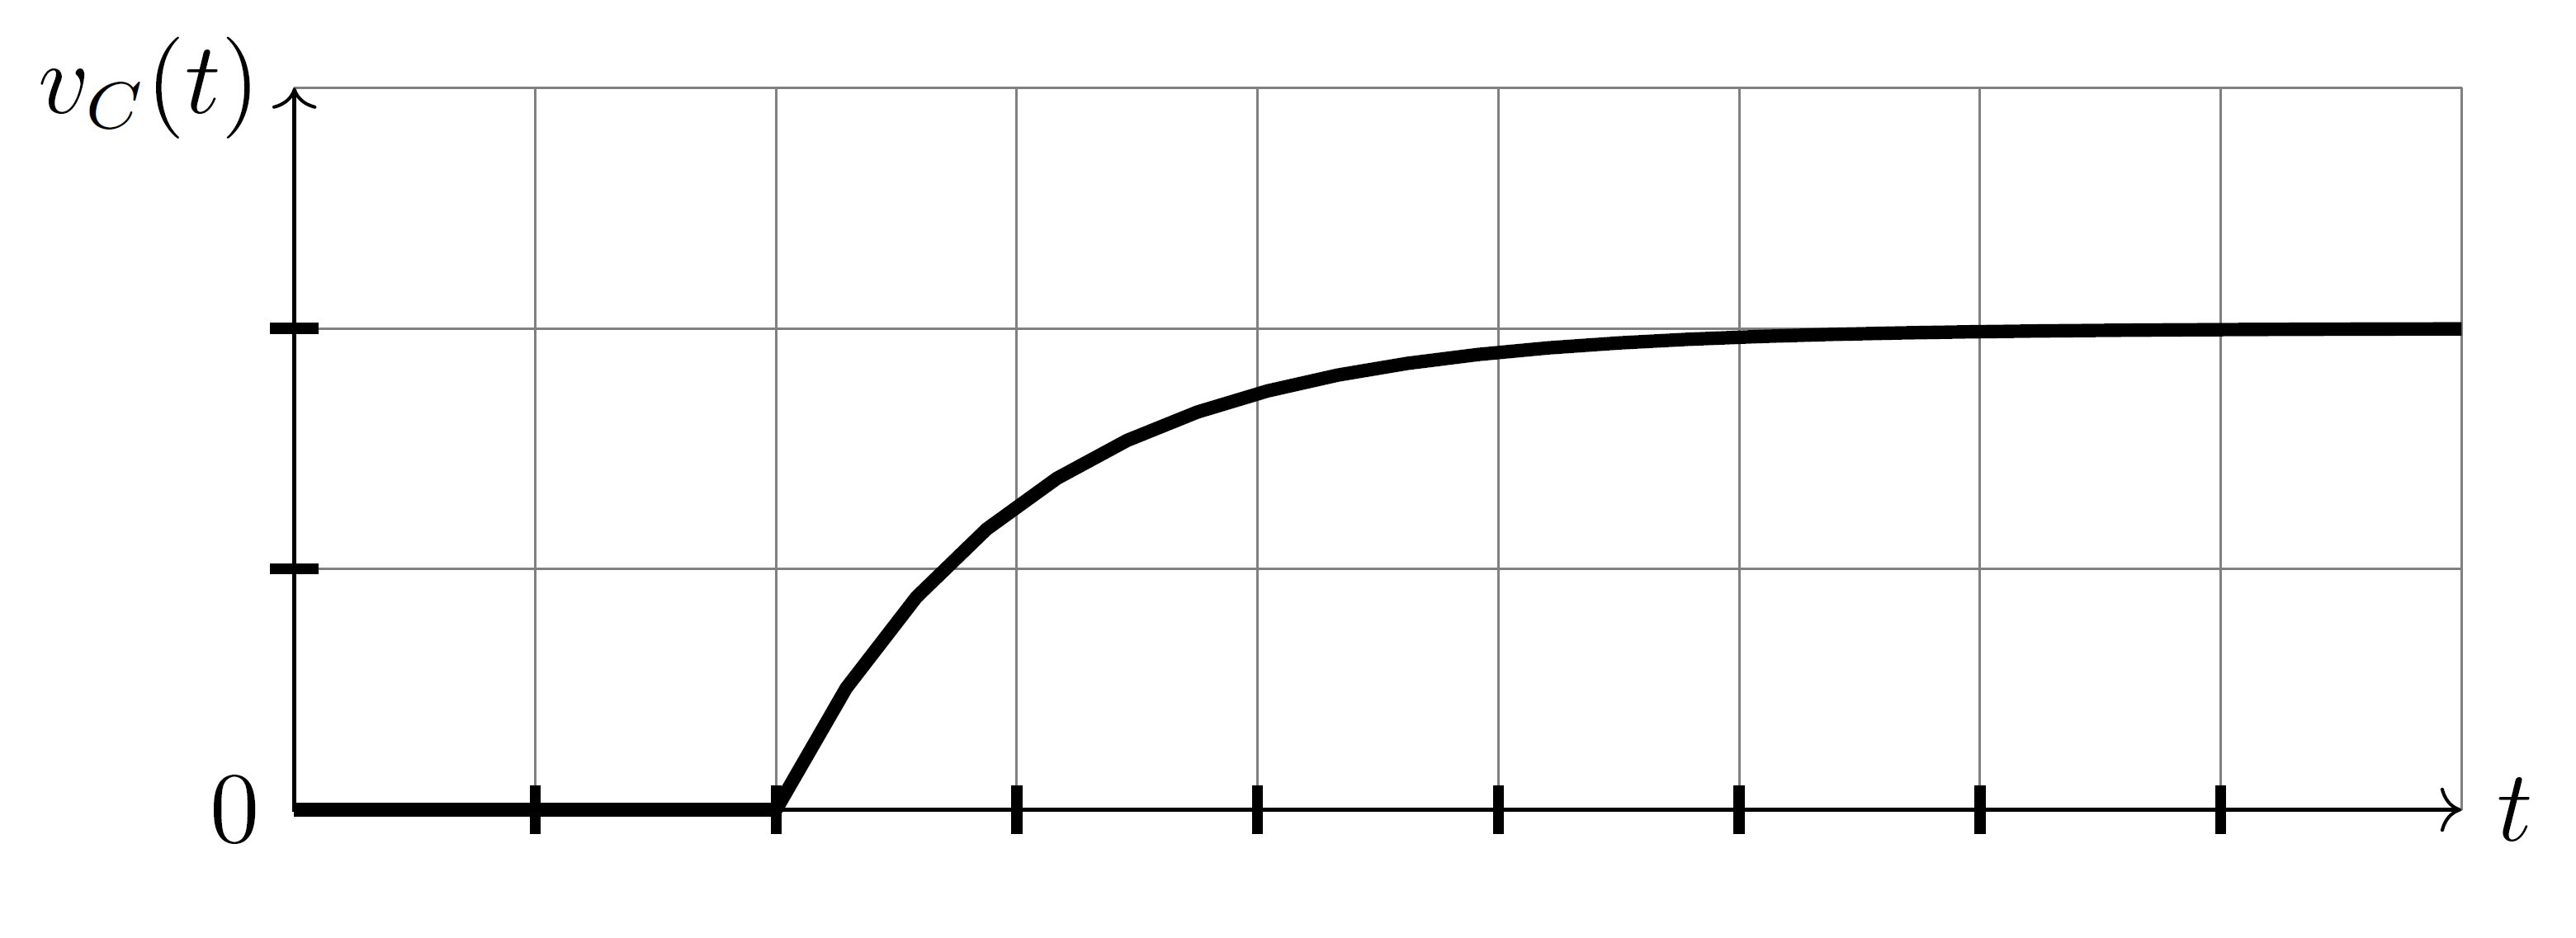
\includegraphics[width=12cm]{files/img4}
\end{center}

\vspace{20px}
\textit{Solución:}
\\

\end{document}